\documentclass[a4paper,12pt]{article}
\usepackage{graphicx}
\usepackage{booktabs}
\usepackage{tikz}
\usepackage{algorithm}
\usepackage{algorithmic}
\usepackage{siunitx}
\usetikzlibrary{shapes.geometric, arrows}

\author{%
Thomas Lam \quad \texttt{z5136612} \\
Akshin Goswami \quad \texttt{z5117650} \\
}
\title{%
The Univerisity of New South Wales \\
\includegraphics[width=0.4\textwidth]{docs/unsw.png} \\
\textbf{COMP2121} \\
\vspace{2.5cm}
Design Manual
}

\tikzstyle{startstop} = [rectangle, rounded corners, minimum width=3cm, minimum height=1cm,text centered, draw=black]
\tikzstyle{io} = [trapezium, trapezium left angle=70, trapezium right angle=110, minimum width=3cm, minimum height=1cm, text centered, draw=black]
\tikzstyle{process} = [rectangle, minimum width=3cm, minimum height=1cm, text centered, text width=3cm, draw=black]
\tikzstyle{decision} = [diamond, minimum width=3cm, minimum height=1cm, text centered, draw=black]
\tikzstyle{arrow} = [thick,->,>=stealth]

\begin{document}
\maketitle
\newpage

\section{Control Flow}
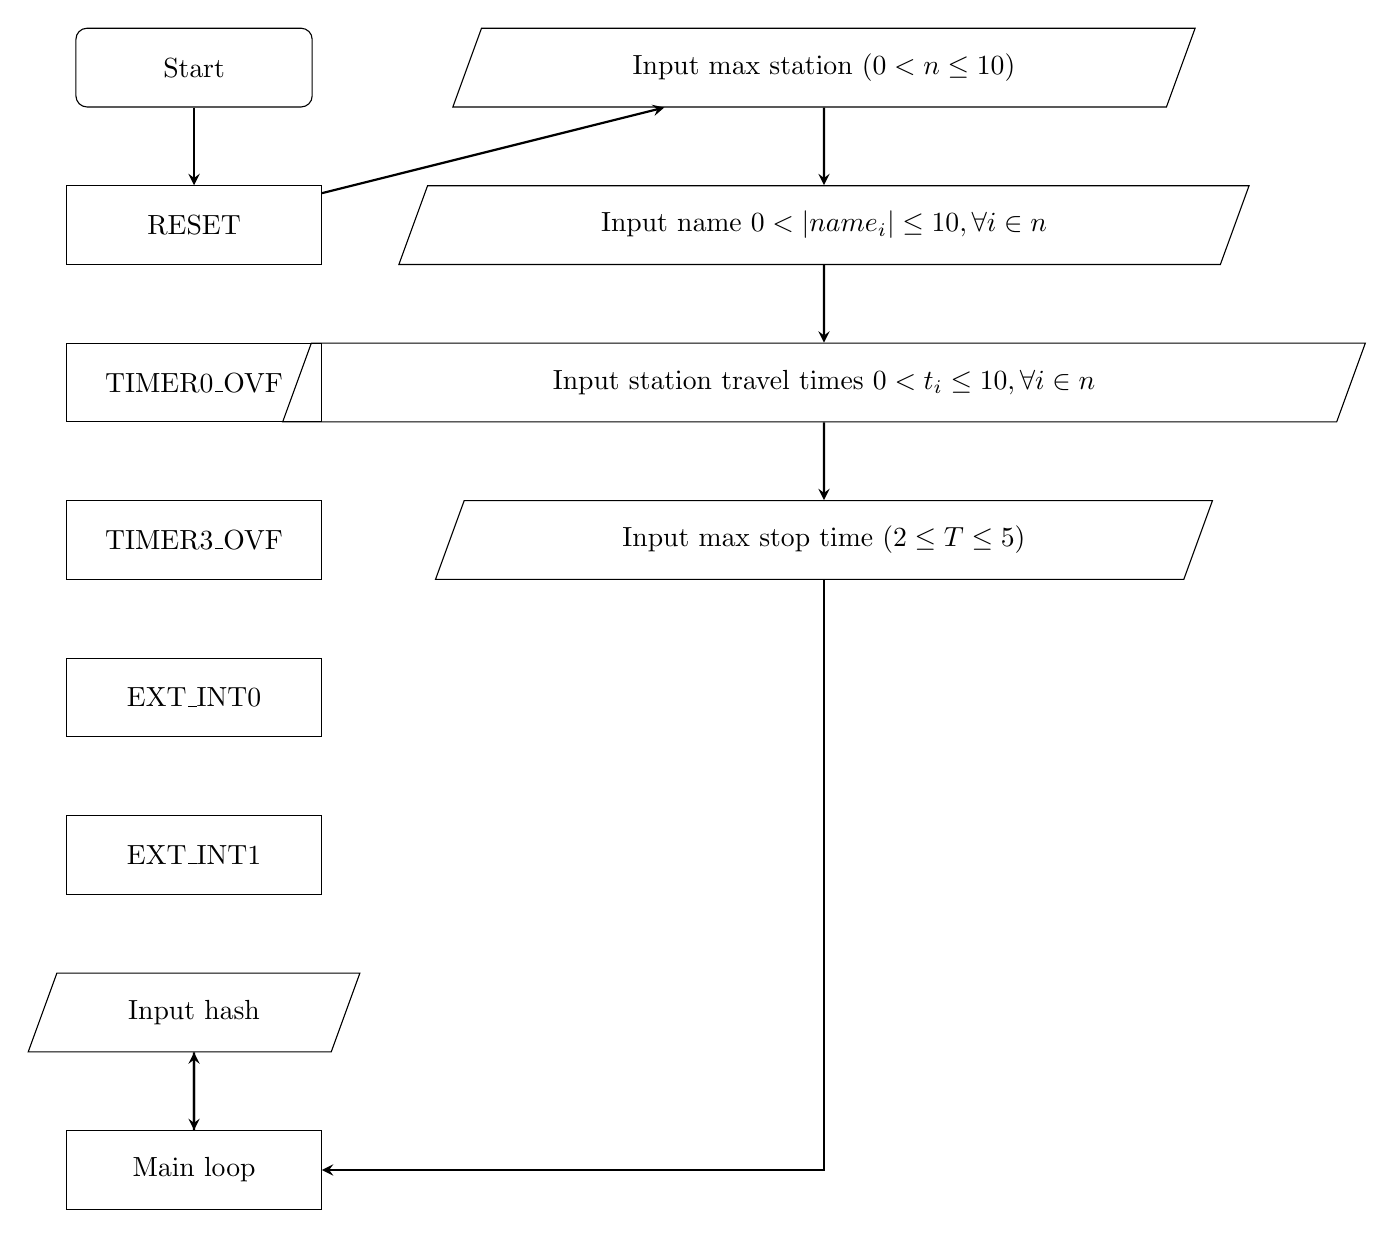
\begin{tikzpicture}[node distance=2cm]\label{fig:flow-chart}
\node (start) [startstop] {Start};
\node (reset) [process, below of=start] {RESET};
\node (in max station) [io, right of=start, xshift=6cm] {Input max station ($0 < n \leq 10$)};
\node (in name) [io, below of=in max station] {Input name $0 < \left\vert name_i \right\vert \leq 10, \forall i \in n$};
\node (in travel times) [io, below of=in name] {Input station travel times $0 < t_i \leq 10, \forall i \in n$};
\node (in max stop time) [io, below of=in travel times] {Input max stop time ($2 \leq T \leq 5$)};

\node (timer0) [process, below of=reset] {TIMER0\_OVF};
\node (timer3) [process, below of=timer0] {TIMER3\_OVF};
\node (extint0) [process, below of=timer3] {EXT\_INT0};
\node (extint1) [process, below of=extint0] {EXT\_INT1};

\node (input hash) [io, below of=extint1] {Input hash};
\node (main loop) [process, below of=input hash] {Main loop};

\draw [arrow] (start) -- (reset);
\draw [arrow] (reset) -- (in max station);
\draw [arrow] (in max station) -- (in name);
\draw [arrow] (in name) -- (in travel times);
\draw [arrow] (in travel times) -- (in max stop time);
\draw [arrow] (in max stop time) |- (main loop);
\draw [arrow] (main loop) -- (input hash);
\draw [arrow] (input hash) -- (main loop);

\end{tikzpicture}

\section{Data Structures}
The simulator stores useful data like the status of the monorail, station names, travel times and stop times.

\begin{table}
    \centering
    \begin{tabular}{lcr}
        \toprule
        Variable & Signature in simluator & Description \\
        \midrule
         max. number of station $n$ &  \texttt{max\_station} & one byte variable \\
         station names $s$ & \texttt{station\_names} & $11 * 10=110$ bytes 2D array \\
         travel time between stations $t_i$ & \texttt{station\_travel\_times} & 10 byte array \\
         stop time in station $T$ & \texttt{stop\_time} & one byte variable \\
         monorail status $\gamma$ & \texttt{stage} & one byte variable \\
         next station & \texttt{to\_station} & one byte variable \\
         stop requests & \texttt{request\_stop} & boolean \\
         seconds left to next action & \texttt{sec\_left} & one byte variable \\
         timer enable & \texttt{enable\_timer} & boolean \\
         timer 0 ovf count $c$ & \texttt{timer0\_ovf\_count} & two bytes variable \\
         timer 0 ovf count for LED $c_{LED}$ & \texttt{timer0\_ovf\_count\_led} & two bytes variable \\
         check if LED is on & \texttt{is\_led\_on} & boolean \\
         \bottomrule
    \end{tabular}
    \caption{Variables in simulator.}
    \label{tab:variables}
\end{table}
Table \ref{tab:variables} shows the type of variables used in the simulator and a brief description of how they are used. Note that $\gamma$ could be one of $\texttt{WAIT\_5}= 1 << 0$, $\texttt{TRAVEL}= 1 << 1$ or $\texttt{STOP}= 1 << 2$.

\subsection{Names of Stations}
The maximum number of stations the simulator can handle is 10 and the character limit of each station name is 10, plus a null terminating character at the end of string. Therefore the array to store all station names is of size $11 * 10 = 110$ bytes.

\section{Algorithms}
\subsection{Character Generation}
Keypad on the board has 16 buttons, of which 8 of them are labelled with letters (3 on each button). That means only $8 \times 3 = 24$ characters\footnote{In fact, Q and Z are missing on the keypad} can be displayed/generated if we were to use this letter pattern in the simulator.

Another problem is that there are only 16 buttons on the keypad, meaning that only 16 unique characters can be generated if each button is ``responsible'' for generating one letter. This is obviously not enough for our use case since we would need to generate 26 English letters plus a whitespace character.

Our solution is to map all 26 English letters from button ``1'' to button ``9'', and generate the space character if button ``0'' is pressed. So for example, button ``1'' is mapped to A, B, C, and button ``2'' is mapped to D, E, F, etc. Note that there is one special case, where button ``9'' is mapped to Y, Z only.

How do we know which character is generated when a button is pressed then? We can use a ``prefix'' button to denote the position of letter we want to output. Since at most 3 letters are mapped to one button, we need 3 prefix buttons. For our simulator, we chose button ``A'', ``B'', ``C'' as prefixes. An example of how this would work: say we want to type ``E'' out, button ``B'' has to be pressed first, then button ``2'', since ``E'' is mapped to position 2 of button 2.

To implement this, we would need a register to store the letter prefix. In the simulator, \texttt{r21} is used. Let $k$ be the key pressed, where $0 \leq k \leq 16$, and $p, 0 \leq p \leq 2$ be the prefix, the character $c$ outputted by the algorithm would be
\[
c = 3(k - 1) + p + 65
\]
Note that 65 is the ASCII code for ``A''. The algorithm could be found in source code \texttt{keypad.inc} labelled \texttt{\_select\_char}.

\subsection{Input Mode Selection}
There are two types of input according to the specification: text input for names, and number input for time and number of stations. Both would require a different input parsing algorithm but the same hardware is used (keypad). Normally two functions are needed to handle two different cases, but in our simulator we reused the same keypad scanning algorithm provided from the labs and lectures. We injected a mode selector to the algorithm and handle the conversion differently according to the input mode.

\begin{algorithm}
\label{alg:input-mode}
\caption{Simple algorithm to handle different input mode}
\begin{algorithmic}
\STATE $key\gets scan()$
\IF {$mode = \texttt{TEXT\_INPUT}$}
    \STATE $handleText(key)$
\ELSE
    \STATE $handleNumber(key)$
\ENDIF
\end{algorithmic}
\end{algorithm}

\subsection{Monorail Simulation}
$\gamma$ is constantly changed in the simulator. Since it, along side with other status-related variables (\texttt{to\_station}, \texttt{request\_stop}) are global static variables, any interrupts/subroutine can change the value of $\gamma$, making it easy for any functions to update the state of the simulator.

In the simulator, \texttt{EXT\_INT1} and \texttt{EXT\_INT0} set \texttt{request\_stop} to true whenever they are triggered. \texttt{TIMER0\_OVF} updates the timer count to check if a particular action has to be handled (depending on $\gamma$). For example, LED is toggled every $\frac{1}{6}$ second\footnote{since LED flashes at $3\si{\hertz}$} if $\gamma = \texttt{STOP}$; monorail is stopped/started if \texttt{sec\_left} is 0.

\subsubsection{Handling LED Flashes}
\texttt{timer0\_ovf\_count\_led} is incremented by 1 every time \texttt{TIMER0\_OVF}. When \texttt{timer0\_ovf\_count\_led} reaches $7812 / 6 = 1302$\footnote{number of timer interrupts in one second $= (1/16000000 \times 256 \times 8)^{-1}\approx 7812$}, LED is toggled.

\subsubsection{Starting the Monorail}
When \texttt{sec\_left} reaches 0 and $\gamma = \texttt{STOP}$, the travel time to the next station is loaded into \texttt{sec\_left}. Name of the next station is displayed on the screen and $\gamma$ is updated to \texttt{TRAVEL}.

\subsubsection{Stopping the Monorail}
When \texttt{sec\_left} reaches 0 and $\gamma = \texttt{TRAVEL}$, the handler checks if \texttt{request\_stop} is set. If it is not, next station is loaded, \texttt{to\_station} and \texttt{sec\_left} are updated to values corresponding to next station. Otherwise $\gamma$ is set to \texttt{STOP} and \texttt{sec\_left} is set to stop time.

An infinite loop runs in main function constantly scan for inputs and check if hash is pressed. If so, monorail is stopped given that $\gamma = \texttt{TRAVEL}$.

\section{Module Specification}
\subsection{\texttt{keypad.inc}}
\begin{itemize}
    \item \texttt{input} convert user input to number or strings. in = mode selector (x register if text mode), out = number input by user if number mode
    \item \texttt{convert} converts button signals to integers.
\end{itemize}
\subsection{\texttt{motor.inc}}
\begin{itemize}
    \item \texttt{motor\_rotate} rotate motor at 60rps. Takes no input and no output.
    \item \texttt{motor\_stop} stop motor rotation. Takes no input and no output.
\end{itemize}
\subsection{\texttt{lcd.inc}}
\begin{itemize}
    \item macro \texttt{prompt\_pm} print string in program memory. in = memory address of string
    \item macro \texttt{print\_str\_2d} print string in a 2D array. in = memory address of string, index, maximum size of string 
\end{itemize}

\section{Board Configuration}
PWM signal would causes the board to reset. To counter this, connect Mot pin to POT pin, and connect JP91 to PE2. Then adjust the potentiometer to tune the motor speed.

\end{document}